\chapter{Introduzione al DDS}
In questo capitolo viene fatta un'introduzione generale dello 
standard del Data Distribution Service (DDS) gestita
dall'Object Management Group (OMG) \cite{8469351}. 
Inizialmente a livello generale 
per poi andare sempre più nel
dettaglio per capire il suo funzionamento. Questo ci sarà utile 
per comprendere le vulnerabilità che verranno analizzate nei
successivi capitoli. Inoltre verrà introdotta la sua estensione 
DDS security che si occupa di rendere più sicuro lo standard DDS 
aggiungendo l'autenticazione e una 
implementazione della cifratura dei pacchetti scambiati tra i vari
dispositivi connessi nella rete. 
Infine verrà mostrato in quali contesti attuali il DDS viene
utilizzato con le sue diverse implementazioni.

In questa tesi potrebbe venire omessa la specifica OMG perché 
faremo riferimento
esclusivamente al DDS conforme all'Object Management Group. Questo 
standard ha delle specifiche tecniche ben precise, consentendo
l'interoperabilità tra i diversi vendor che lo rispettano, insieme
a tanti altri numerosi vantaggi \cite{dds1.4}.


\section{Modello publish/subscribe}
Prima di parlare del DDS, è necessario capire il 
funzionamento del modello Publish-Subscribe 
che sta alla base del suo funzionamento.
Questo modello di publish e subscribe non funziona come la 
classica applicazione che siamo abituati a vedere tra server e
client tramite protocollo TCP/IP nell'ambito delle comunicazioni. 


\subsection{Perché non usiamo una connessione con TCP/IP}
Prendiamo l'esempio di un collegamento tra una workstation e 
un sensore per la temperatura. La connessione a livello fisico
avverrà tramite un collegamento Ethernet. La workstation e il 
sensore quindi si trovano nello stesso network e possono 
ora cominciare a comunicare tra di loro. L'obiettivo è quello
di trasferire i dati dal sensore alla workstation in modo tale
da poterli visualizzare a schermo.
La metodologia più frequente è quella di utilizzare un socket tramite 
protocollo TCP/IP, ma non sempre questa è la soluzione migliore.
Alcuni vantaggi del TCP/IP sono la disponibilità di utilizzo 
in molte applicazioni e nella maggior parte 
delle connessioni a Internet.
Tuttavia, in certe implementazioni, TCP/IP non risulta la soluzione migliore,
specialmente quando dobbiamo collegare un numero di dispositivi al 
network che può variare nel tempo. Se nel nostro network tra workstation e 
sensore della temperatura, aggiungiamo un altro dispositivo, ad esempio un 
sensore per la temperatura, bisognerebbe creare un nuovo socket 
TCP/IP per far comunicare il nuovo sensore con la workstation.
Questo è necessario perché TCP/IP supporta una comunicazione di tipo 
one-to-one (uno a uno). Come vedremo nella prossima sottosezione,
il modello publish/subscribe non ha questa limitazione \cite{1494965}.



\begin{figure}[H]
    \centering
    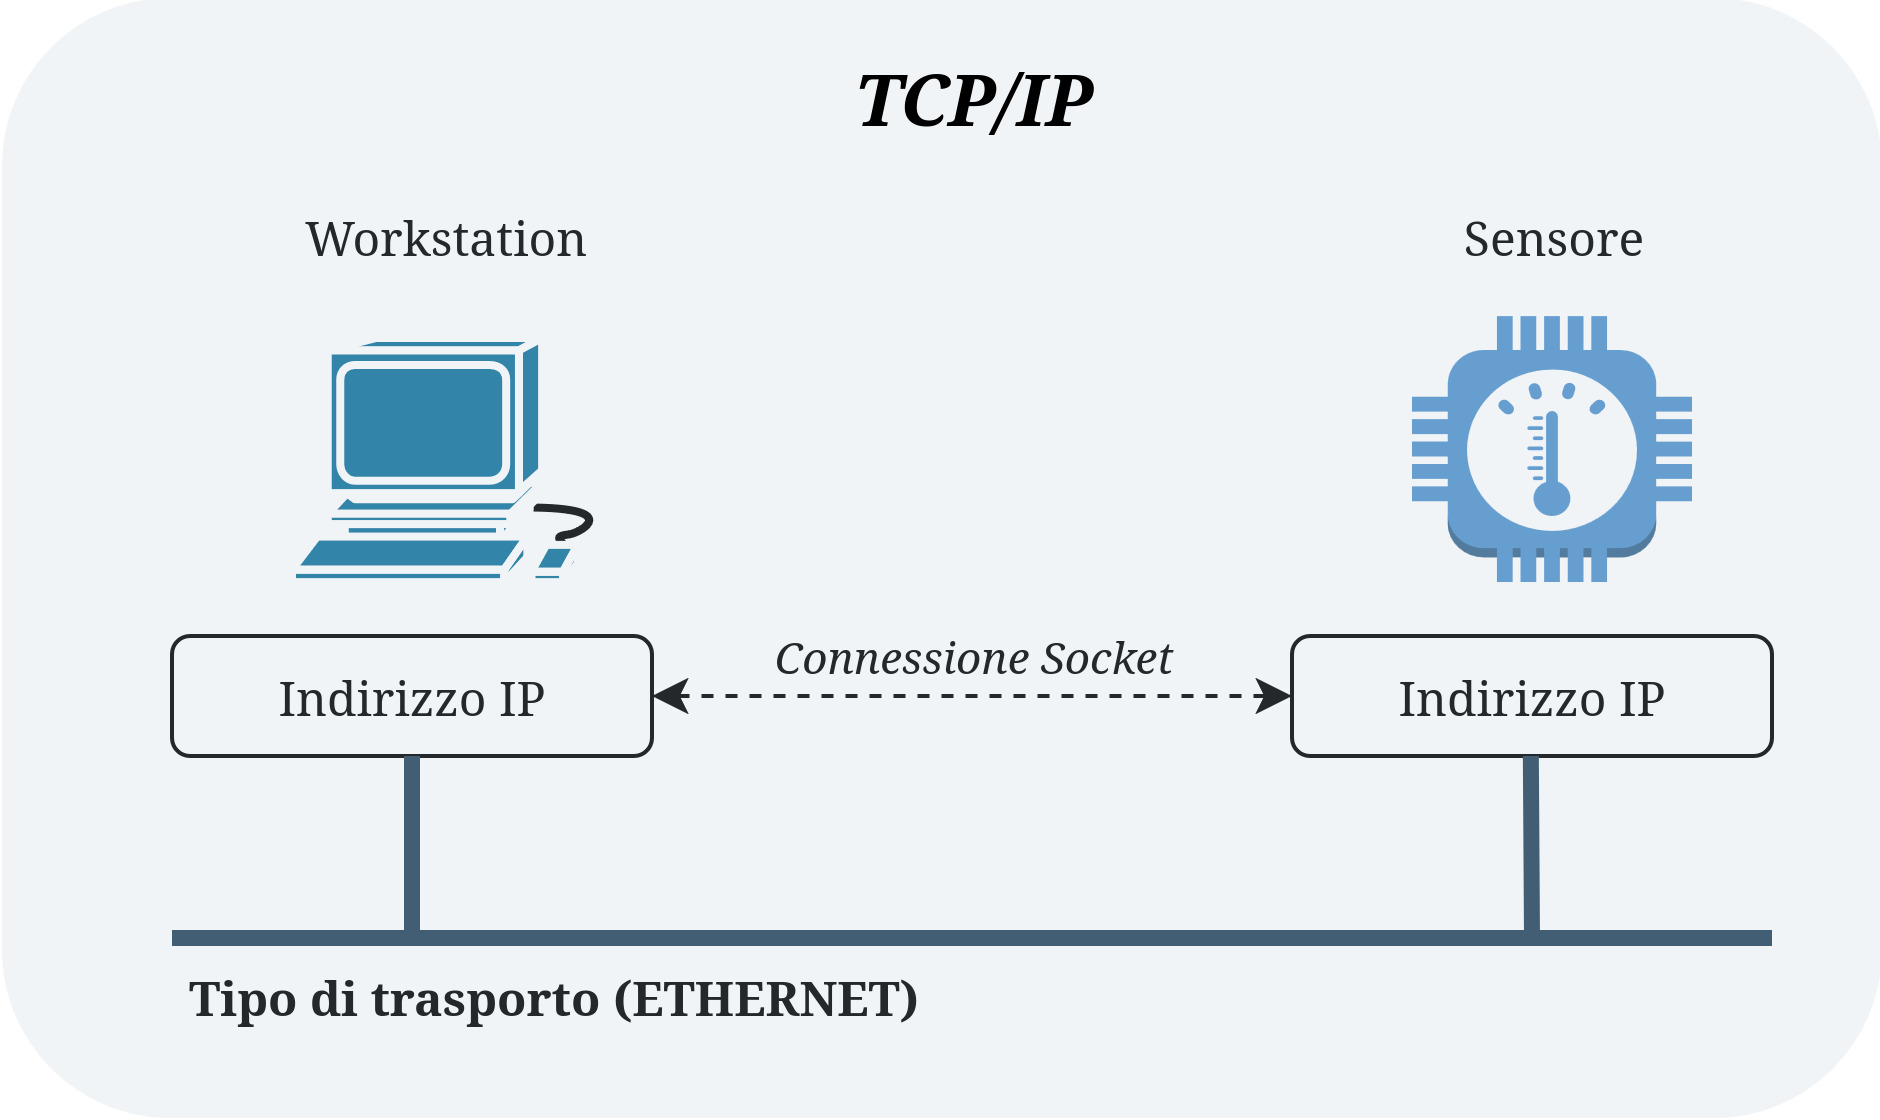
\includegraphics[width=12cm, keepaspectratio]{img/TCP connessione-Pagina-2.jpg}
    \caption{Un esempio di collegamento tra una workstation e un sensore della temperatura,
    utilizzando il protocollo TCP.}
    \label{TCP connection}
\end{figure}



\subsection{Struttura modello publish/subscribe}
% Citazione da mettere
Per funzionare, il modello publish/subscribe, ha bisogno di
due elementi chiamati publisher e subscriber, 
che permettono lo scambio di messaggi all'interno del network.
La comunicazione avviene 
quando hanno un topic, che
rappresenta una tipologia di dati (ad esempio la temperatura, 
la distanza e la velocità) è in comune tra di loro.
\begin{itemize}
    \item Publisher: colui che pubblica nuovi dati riguardanti dei
    topic rendendoli accessibili ai subscriber iscritti. 
    Di solito si tratta di un sensore.
    \item Subscriber: è colui che si iscrive ai topic del publisher, 
    cominciando
    così a ricevere nuovi dati sul topic scelto. Spesso si tratta
    di un dispositivo utilizzato per visualizzare informazioni, come uno
    schermo.
\end{itemize}
Chiamiamo entità tutti i dispositivi che fanno parte del modello 
publish/subscribe.
Una caratteristica di queste entità è che possono essere aggiunte o rimosse
da una rete senza nessun problema, dato che le 
comunicazioni avvengono in modalità asincrona \cite{dds1.4}. 

Inoltre questo modello risulta molto
flessibile e adatto in ambienti real-time dove le informazioni
possono cambiare o essere utilizzate da più dispositivi.
I subscriber, ad esempio possono cambiare i topic a cui 
sono iscritti e i publisher possono smettere di pubblicare nuovi
aggiornamenti su un determinato topic anche a runtime \cite{OH2010318}.

\section{Che cos'è il Data Distribution Service}

Il DDS gestito da OMG è un middleware e uno standard API con una gestione
dei dati di tipo data-centric. 
Prendendo in considerazione il modello ISO OSI 
(Open Systems Interconnection), questo
middleware è un software che si trova tra l'applicativo e il livello
del trasferimento.

\begin{figure}[H]
    \centering
    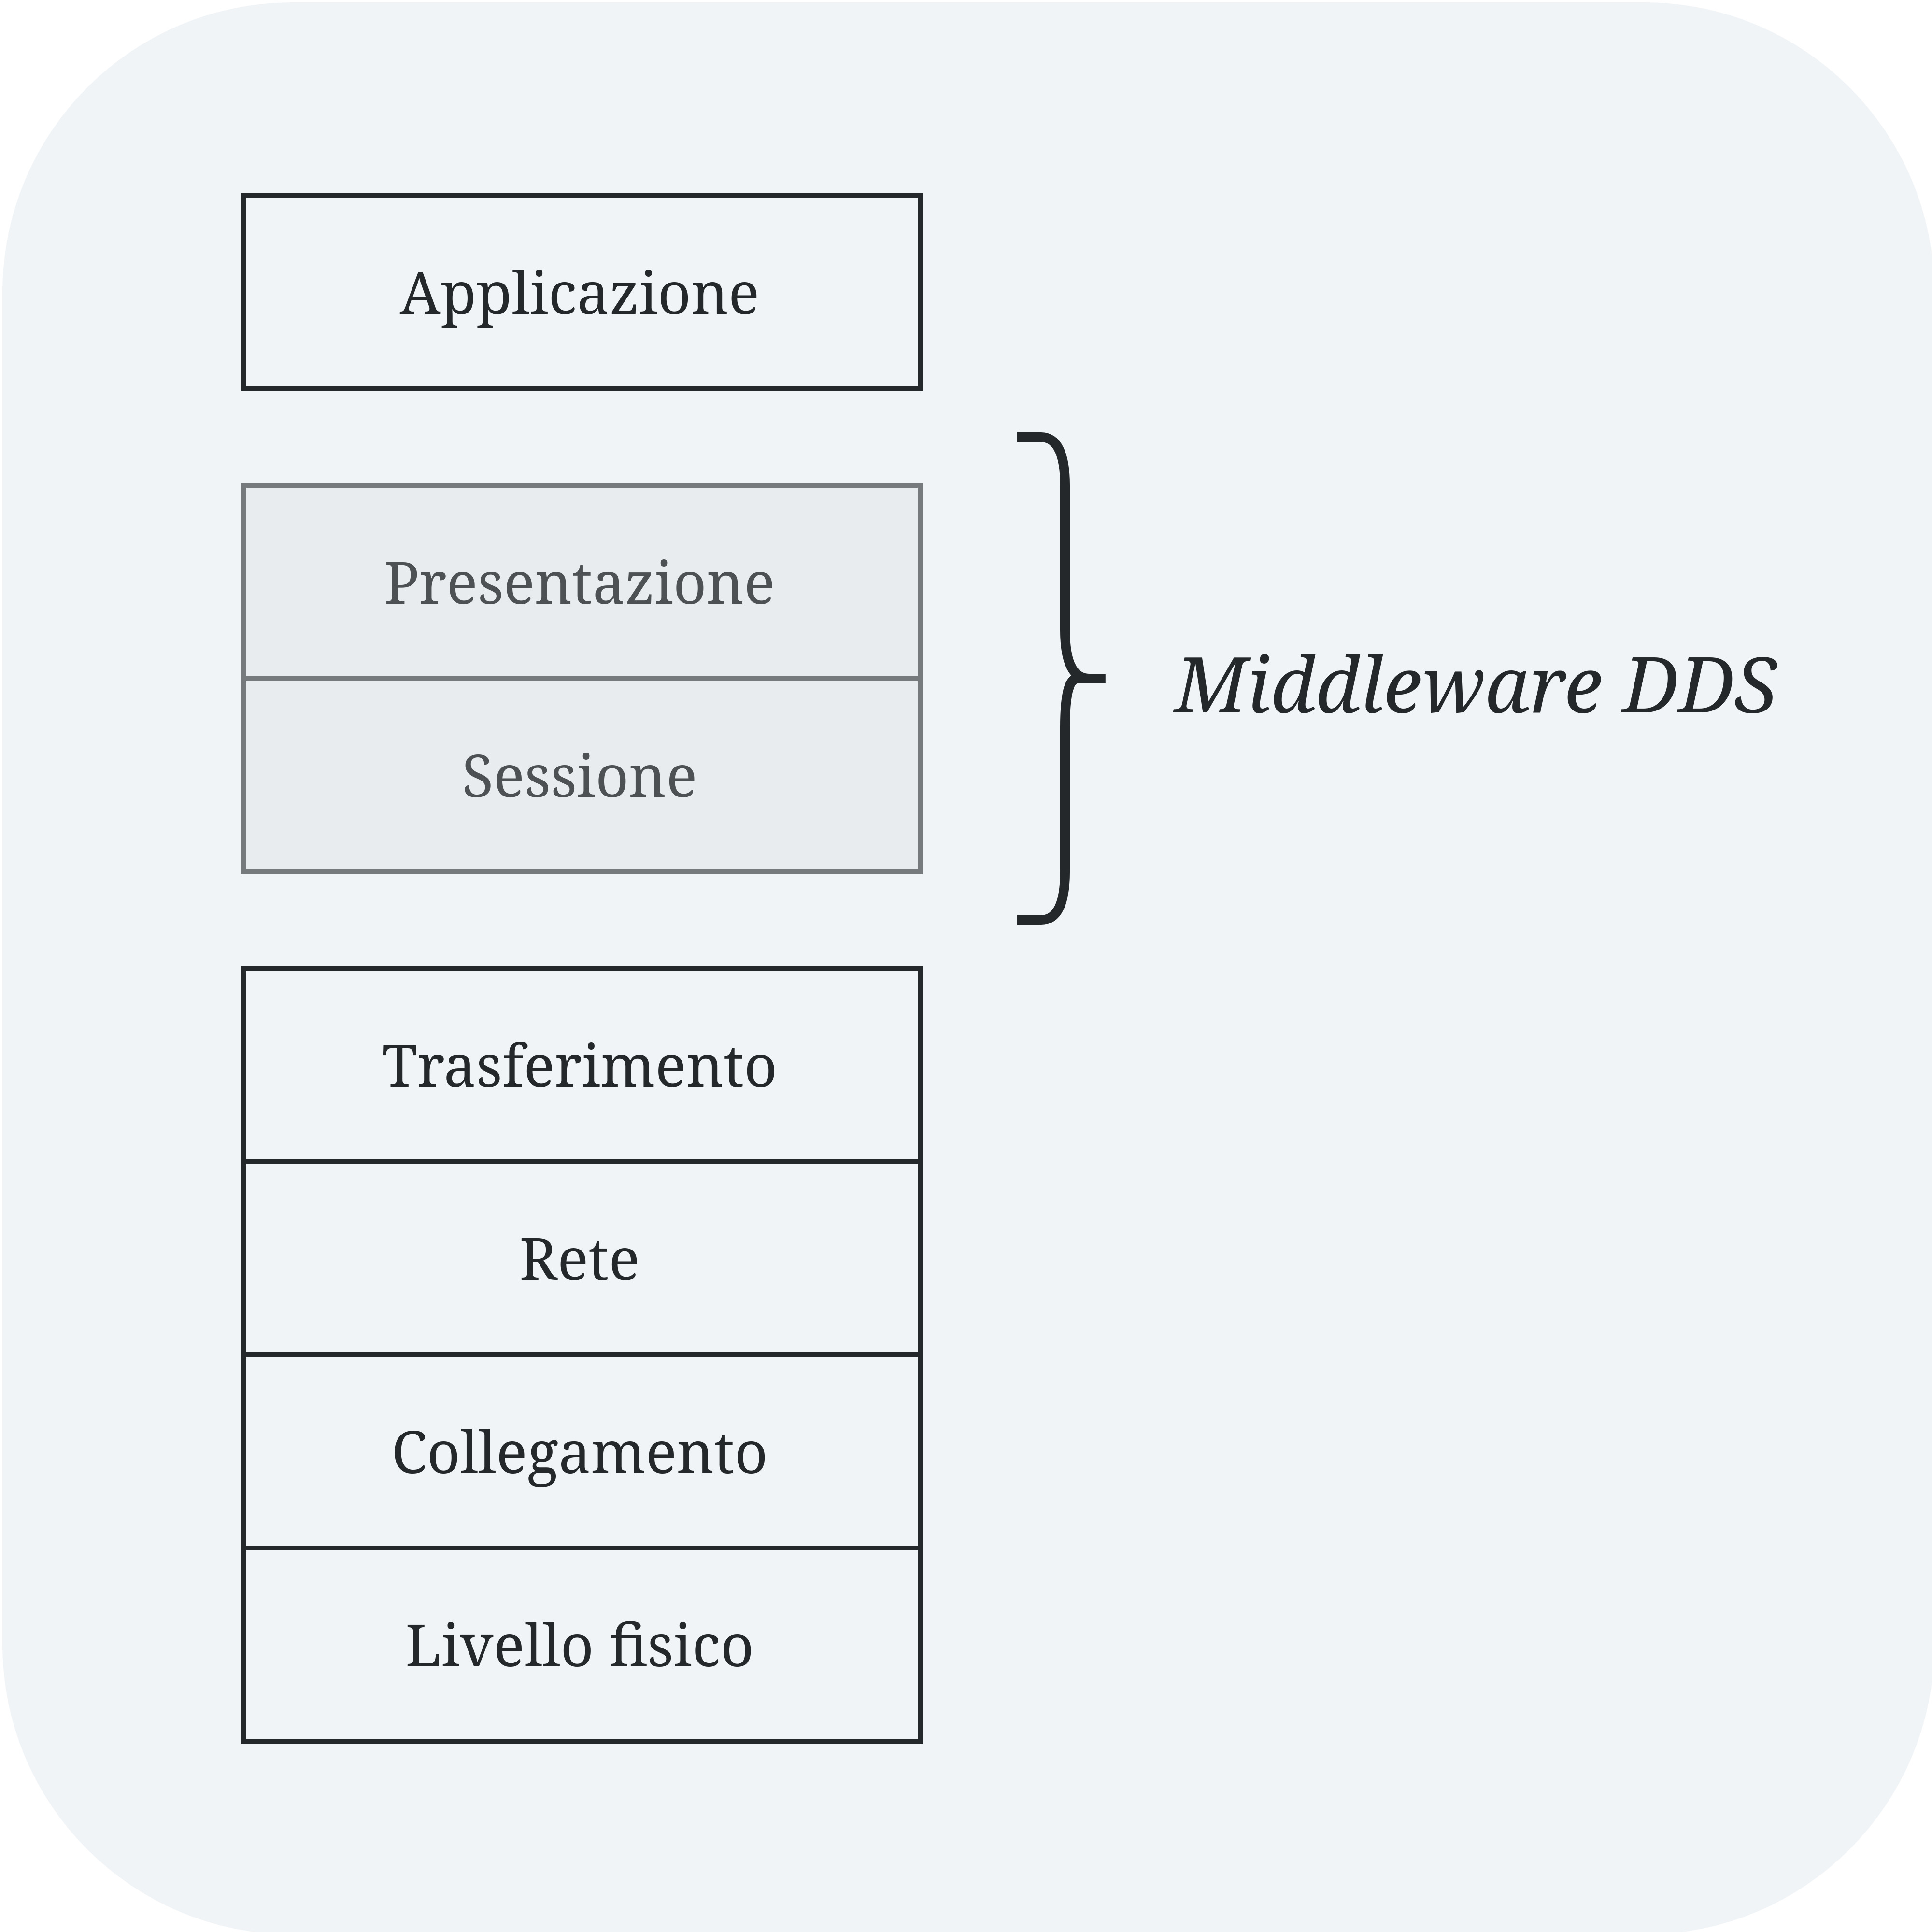
\includegraphics[width=10cm, keepaspectratio]{img/ModelloISOOSIDDS-Pagina-3.jpg}
    \caption{Posizione del middleware DDS nel modello ISO/OSI.}
    \label{DDSISOOSI}
\end{figure}


% fare disegno layers osi
Il DDS si basa sul DCPS (Data-Centric Publish-Subscribe) 
che è un modello di comunicazione simile a quello
di tipo publish/subscribe, ma con un approccio più data-centric, in modo
tale da semplificare il lavoro del programmatore che si deve solamente
occupare di specificare il contesto del dato che deve mandare o ricevere.
Con data-centric infatti, specifichiamo che il focus del modello DCPS 
è incentrato 
sui dati stessi, anziché sulle entità che li scambiano \cite{whatisdds}.
Così facendo non bisogna preoccuparsi dell'invio o della ricezione
dei messaggi, perché questa parte viene completamente gestita dal middleware.
% Il DDS è stato il primo standard
% a formalizzare le comunicazioni di tipo data-centric. Inizialmente erano 
% disponibili solamente soluzioni proprietarie senza specificare un standard
% univoco. Non avendo avuto uno standard univoco le varie implementazioni dei vendors
% non erano
% compatibili tra di loro a differenza del DDS.

% Magari fare la differenza tra data centri e message centric

Altri vantaggi del DDS includono una architettura adattabile che supporta
degli elementi di auto-scoperta (auto-discovery) o Dynamic Discovery 
in modo tale da aggiungere o 
rimuovere dispositivi dalla rete in modo automatico, anche a runtime.
Il Dynamic Discovery ha il compito di analizzare quali tipologie di dati 
ha bisogno questo nuovo dispositivo. 

Inoltre ogni nuovo partecipante 
utilizzerà sempre le stesse API per comunicare con l'applicativo dato che 
non c'è bisogno di configurare le impostazioni degli indirizzi IP o 
preoccuparsi delle diverse architetture \cite{1494965}.
 
 
\subsection{Quality of Service (QoS)}

Per soddisfare i diversi requisiti di una trasmissione dati, 
il Data Distribution Service (DDS) utilizza un insieme di policy
Quality of Service (QoS). Queste policy permettono di controllare, 
regolare e ottimizzare lo scambio di dati tra i vari componenti 
all'interno del middleware. Queste policy QoS possono variare 
significativamente in base al tipo di comunicazione richiesta, 
offrendo una gestione altamente flessibile e granulare. 
Ogni elemento del middleware può essere configurato 
con policy specifiche, in modo tale da adattarsi alle 
esigenze dell'applicazione.

\subsection{Global Space Data}
Il DDS utilizza il Global Data 
Space (spazio dati globale), un'area logica condivisa 
che consente agli applicativi
di accedere a una sorta di memoria locale tramite API.
L'applicativo nella scrittura o nella ricezione dei dati utilizzerà 
questa memoria locale fittizia assumendo il ruolo di 
un'unica risorsa centralizzata.
Tuttavia, i dati all'interno di questa memoria possono contenere
informazioni provenienti da nodi remoti distribuiti per la rete. 
L'applicativo non deve cosi preoccuparsi dell'accessibilità dei dati,
poiché questi vengono gestiti agendo come se si trovassero tutti in unico punto 
\cite{whatisdds}.


\subsection{Architettura DDS}
Lo standard DDS definito dall'OMG è composto da due layer: 
il DDS e il
DDSI (DDS Interoperability).
    \begin{itemize}
        \item DDS: è il layer fondamentale in cui troviamo il DCPS
        (Data-Centric Publish-Subscribe),
        il modello di comunicazione simile a quello di tipo publish/subscribe,
        che si occupa di mettere in comunicazione più applicazioni 
        tra di loro. In questo layer vengono inoltre 
        definite le policy QoS \cite{Michaud2017Apr}.
        \item DDSI: è il layer che si occupa di garantire l'interoperabilità
        tra le diverse implementazioni del DDS, ad
        esempio quando provengono da vendors diversi.
        All'interno di questo layer troviamo l'RTPS 
        (Real-Time Publish-Subscribe Protocol), un protocollo che permette ai 
        vari dispositivi DDS di comunicare e scoprirsi tra di loro
        (Dynamic Discovery).
        RTPS è il wire-protocol (un protocollo che permette lo scambio di 
        messaggi del DDS al layer di trasporto di rete 
        del modello ISO OSI) ufficiale del DDS, 
        con standard definito da OMG,
        che definisce il formato dei messaggi e impone le regole che 
        permettono una trasmissione standardizzata di scambio dati. 
        Se questo wire-protocol non fosse presente,
        le diverse implementazioni del DDS non potrebbero 
        comunicare tra di loro \cite{essay93639}.
    \end{itemize} 



% \subsection{Dynamic Discovery}
% \cite{whatisdds}




% \subsection{In che contesti viene utilizzato e perché}

% \subsection{Versioni DDS}



% Schema layer middleware

% https://www.dds-foundation.org/what-is-dds-3/

\section{Le entità del DCPS}
Il layer DDS per operare utilizza le entità definite dal DCPS, 
che rappresentano gli elementi necessari
per il funzionamento dell'intero middleware. Queste hanno il compito di 
gestire i dati
scambiati tra i vari partecipanti all'interno del sistema. 
Le entità principali del DDS sono: 
il publisher, il subscriber, il DataWriter, il DataReader, il Topic,
la Istanza, il Domain e il Domain Participant.
Ognuna di queste entità deve tener conto del suo set di policy 
QoS configurate
che ne definiscono il comportamento. Queste policy verranno analizzate 
più nel dettaglio nella Sezione~\ref{Le policy QoS nel dettaglio}.
% Aggiungere riferimento

\begin{figure}[H]
    \centering
    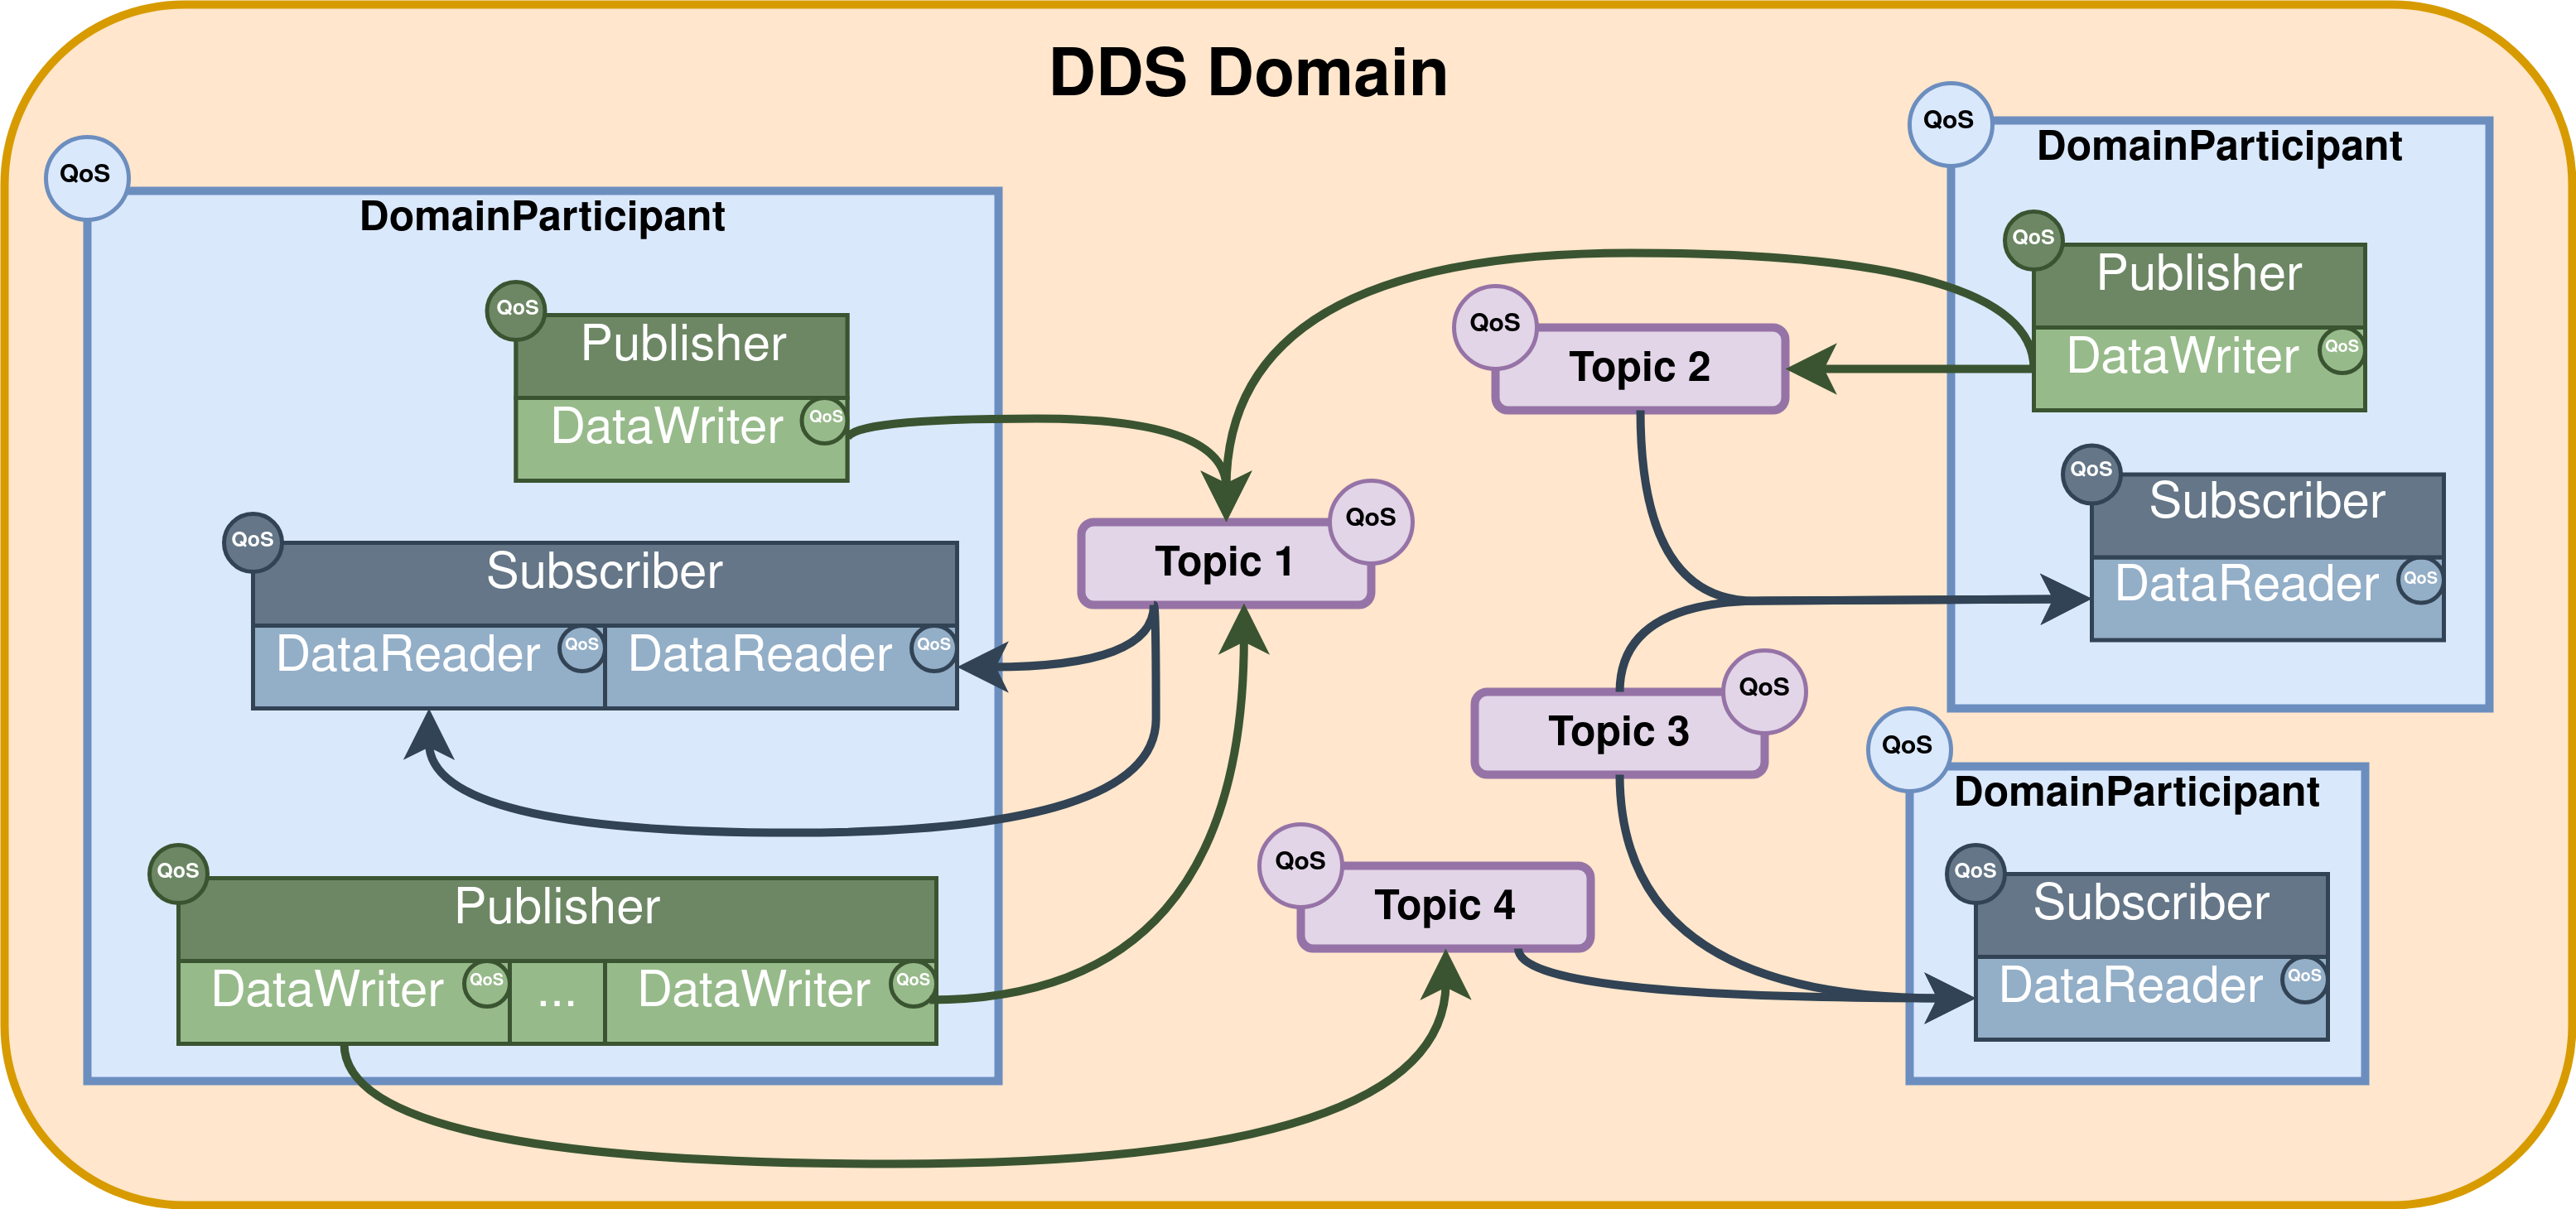
\includegraphics[width=15.2cm, keepaspectratio]{img/entitadcps .png}
    \caption{Entità DCPS del DDS. 
    Fonte: \cite{whatddseprosima}}
    \label{entitadcps}
\end{figure}



Il linguaggio utilizzato da queste entità si chiama Interface 
Definition Language (IDL) e anch'esso è standardizzato da OMG. 
IDL è un linguaggio tipizzato 
simile a C++ che supporta i seguenti data types: char, octet, short,
unsigned short, long, unsigned long, long long, unsigned long long, 
float, double, long double, boolean, enum, array e string
\cite{1494965}.


\subsection{Publisher e Subscriber}
Publisher e subscriber sono entità che abbiamo già incontrato
in precedenza nel modello publish/subscribe. Queste due entità 
mantengono lo stesso ruolo all'interno del modello DCPS.

\subsection{DataWriter e DataReader}

Per comunicare tra loro, un publisher si interfaccia tramite
DataWriter, 
mentre il subscriber si interfaccia tramite un DataReader.
Il DataWriter e il DataReader sono interfacce, 
perché l'applicativo
può mandare e ricevere dati
tramite queste due entità fondamentali. 
Questi dati scambiati tra middleware e applicativo
sono i data type e i data-values. I data type consentono di 
descrivere la struttura e il formato del dato, mentre i data-value
sono i dati veri e propri che rispettano le specifiche data type.
\begin{itemize}
    \item DataWriter: è l'interfaccia usata dagli applicativi 
    per spedire i
    data-values con un loro specifico data type ai publisher.
    Ricevuti questi data-values il publisher spedirà le
    informazioni ricevute dall'applicativo ai relativi subscriber.
    \item DataReader: è l'interfaccia usata dagli applicativi per
    ricevere i data-values con i rispettivi data type pubblicati in
    precedenza da un publisher \cite{dds1.4}.
\end{itemize}
È possibile
associare più DataReaders ad un unico publisher e più DataWriters ad
un unico subscriber. Tuttavia, un DataWriter può essere associato solo ad un 
Publisher e un DataReader solo ad un Subscriber. 
Questo avviene perché
i DataReaders e DataWriters possono utilizzare un solo data type alla volta, 
mentre 
i publisher e i subscribers, non avendo questa limitazione, possono gestire 
più DataWriters e DataReaders alla volta.

% Inserire immagine

\subsection{Topic}
% Specificare dove sono stati introdotti
Nel modello publish/subscribe abbiamo già introdotto i topic, ma 
abbiamo la necessità di approfondirli quando vengono utilizzati
con le specifiche del DDS.

I topic vengono utilizzati per identificare il data type
scambiato tra i publishers e i subscribers, creando cosi un punto
di connessione 
tra DataWriter e DataReader \cite{topicomg}.
All'interno del topic troviamo il nome,
i data types e le policy QoS.
Il nome del topic corrisponde ad una stringa univoca 
che serve per identificarlo 
tra gli altri topic del domain.


\subsection{Key e Istanza}
Uno o più data types di un topic possono diventare la chiave (key) del topic. 
Queste chiavi ci permettono di suddividere
i data-values di un topic, dividendoli a seconda della chiave.
Ogni suddivisione che effettuiamo tramite una key diversa crea 
un'istanza che al suo interno contiene i data-values di un 
flusso di dati (data-stream)
\cite{Instance81:online}.

Per fare un esempio prendiamo il topic velocità in un contesto dove si
vogliono analizzare i dati di una gara.
La struttura del topic avrà due data types: il primo corrisponde al valore
della velocità registrata, mentre il secondo mostra l'id-macchina 
che identifica da quale vettura i dati provengono.

\vspace{5mm} % Riusare per codici futuri
\begin{lstlisting}[language=C++, caption=Esempio di Topic con una key
    usando il linguaggio IDL.
    , label=topic struct,
    captionpos=b]
struct Veicolo { // Nome del topic
    id_macchina; // Key del topic
    velocita;
}
\end{lstlisting}
\vspace{5mm}

Creiamo ora due istanze, una con valore 270 per la velocità e con 
l'id-macchina uguale a 1 e l'altra con un valore di 220 per la velocità e 
con id-macchina 
uguale a 2. L'id-macchina fungerà da key 
del topic per distinguere la provenienza dei dati; in questo
modo possiamo così controllare le due macchine con due istanze ciascuna.
\
% Magari anche con RTI shapes
\label{Key e Istanza}

\subsection{Domain}
L'entità del domain (dominio) rappresenta uno spazio logico definito che
ha lo scopo di mettere in comunicazione i vari applicativi tra di loro.
All'interno possiamo trovare i vari topic che collegano gli applicativi
con i loro rispettivi data-types.
L'entità domain è caratterizzata dalle seguenti proprietà:
\begin{itemize}
    \item Ogni domain viene identificato da un id 
    per renderlo univoco.
    \item Ogni entità del DDS può appartenere
    ad un solo domain.
    \item Le entità all'interno del domain possono interagire
    solamente con le altre entità all'interno dello stesso domain
    \item Due applicativi DDS per poter comunicare tra di loro
    hanno bisogno di entrare nello stesso domain.
    \item Un applicativo può far parte di più domain creando 
    più istanze dell'entità DomainParticipant in ogni
    domain in cui vuole interagire \cite{domainrti}.
\end{itemize}

% (possibilità di aggiungere esempi con demo shapes)

\subsection{DomainParticipant}
L'entità del DomainParticipant all'interno di un Domain del DDS,
viene utilizzata dagli applicativi e 
rappresenta la prima entità creata da un'applicazione che verrà 
impiegata per creare DataWriters e DataReaders. 
Questa entità ha il compito di inizializzare
le comunicazioni con il Domain attraverso 
il processo di discovery.
Questo processo consente alle entità appartenenti allo 
stesso domain di trovarsi e connettersi automaticamente.
% Processo discovery non ancora introdotto
L'entità DomainParticipant è caratterizzata dalle seguenti proprietà:
\begin{itemize}
    \item Il DomainParticipant come le altre entità, può 
    esistere solo all'interno di un dominio.
    \item Il DomainParticipant è responsabile della scoperta di altri
    DomainParticipant all'interno del domain \cite{domainparticipantrti}.
\end{itemize}


\section{Le policy QoS nel dettaglio}
A livello logico, le specifiche del DDS
definiscono un insieme di policy QoS
che le entità del DCPS devono rispettare. Qui di seguito vengono
proposte le categorie QoS più rilevanti.
\begin{itemize}
    \item Ownership: questo valore specifica se un topic
    può essere aggiornato da più 
    (SHARED ownership) o da un solo (EXCLUSIVE ownership) publisher.
    Se abbiamo impostato un ownership di tipo EXCLUSIVE, per decidere il 
    publisher che ha la possibilità di aggiornare il topic, viene 
    utilizzato l'ownership STRENGTH.
    \item Liveness: viene utilizzato per specificare se è necessaria
    una comunicazione di tipo attivo, rispetto ad una di tipo 
    intermittente.
    \item Reliability: specifica se in una comunicazione tutti i dati
    trasferiti tra publisher e subscriber devono essere consegnati
    per intero, oppure
    se è accettabile anche la perdita di alcuni dati.
    \item Lifespan: specifica il tempo di scadenza dei dati pubblicati da 
    un publisher.
    \item History: specifica quanti e come i dati devono essere 
    mantenuti in un 
    subscriber dopo averli ricevuti.
    \item Durability: specifica se i dati inviati in precedenza sono
    disponibili per i nuovi subscriber appena entrati nel domain.
\end{itemize}
Le configurazioni 
delle policy vengono trasmesse alle varie entità dal DomainParticipant
tra cui i publisher, i subscriber, i topic e i DataWriters.
Tuttavia, le policy di un publisher e un subscriber devono essere compatibili.
Se così non fosse, la comunicazione tra i due potrebbe essere compromessa
\cite{Michaud2017Apr}.
\label{Le policy QoS nel dettaglio}


\section{Il protocollo RTPS}
RTPS (Real-Time Publish-Subscribe Protocol) è il wire-protocol 
nativo utilizzato dal DDS che consente di trasferire i dati provenienti
dal layer DDS a quello di trasporto della rete.
Solitamente questo viene utilizzato in combinazione con il protocollo
best-effort
UDP/IP, che risulta ottimale per le comunicazioni di tipo real-time. Tuttavia 
anche i protocolli connection-oriented incluso il TCP/IP possono essere utilizzati. 
RTPS include molti vantaggi ideali per il DDS:
\begin{itemize}
    \item Connettività plug and play: le nuove applicazioni possono unirsi o 
    lasciare il domain a proprio piacimento.
    \item Tolleranza ai guasti: non sono presenti singoli punti di 
    guasto perché i dati vengono distribuiti e replicati tra le varie 
    entità DDS che adoperano il Global Data Space.
    \item Type-safety: gli errori di programmazione vengono gestiti 
    in modo tale da non compromettere il funzionamento 
    dei dispositivi remoti.
\end{itemize}
L'RTPS è suddiviso in quattro moduli differenti: lo structure module, il 
messages module, behavior module e il discovery module \cite{ddsrtps}.

\subsection{Structure and behavior module}
Lo structure module si occupa di associare le entità DDS alle corrispondenti
entità RTPS. Queste entità RTPS sono utilizzate 
per rappresentare le entità del DDS (come DataReader e DataWriter) 
all'interno del protocollo RTPS (come l'RTPS Writers e l'RTPS Readers) 
\cite{ddsrtps}.

Il behavior module, invece, definisce le regole di comunicazione tra
due o più entità RTPS, che sono i RTPS Writers e i RTPS Readers 
(definite dal behavior module), durante 
una sequenza di messaggi.
Esse consentono di mantenere l'interoperabilità tra le varie 
implementazioni (anche di diversi vendors) del DDS \cite{ddsrtps}.

\subsection{Messages module}
Il messages module si occupa di descrivere il formato dei messaggi scambiati
tra i RTPS Writers e i RTPS Readers che sono composti da un header
seguito da dei sottomessaggi (Figura~\ref{wireskartshapesdemo}). 
Nell'header troviamo informazioni relative al
protocollo RTPS, cioè la sua versione, il nome del vendor dell'implementazione
usata e il mittente. Nel sottomessaggi invece possiamo trovare un header
e una serie elementi. Nell'header del sottomessaggio
è presente l'id che ne
identifica il tipo, eventuali flag e la lunghezza in bytes 
del sottomessaggio stesso. Le tipologie dei sottomessaggi più importanti, 
identificate dal suo header, sono:
\begin{itemize}
    \item DATA: in questo sottomessaggio vengono trasferiti dall'RTPS Writers
    all'RTPS Reader i dati effettivi relativi ad un topic.
    \item HEARTBEAT: viene mandato da un RTPS Writer a un RTPS Reader per 
    comunicare il numero di nuovi (sequence number) aggiornamenti che il 
    Writer ha disponibili.
    \item ACKNACK: utilizzato per comunicare lo stato di un RTPS Reader 
    al corrispondente RTPS Writer e per informarlo riguardo i dati ricevuti
    e quelli mancanti. Questo sottomessaggio, con la flag FINAL 
    impostata, consente di far rimanere il Reader sincronizzato con l'RTPS
    Writer \cite{ddsrtps}.
\end{itemize} \label{Messages module}


\subsection{Discovery module}
Questo modulo garantisce che i nuovi partecipanti DDS (publisher e subscriber)
riescano a identificarsi in automatico tra di loro in modo tale da inizializzare una 
possibile comunicazione. Questo modulo è responsabile dell'auto-scoperta 
(Dynamic Discovery)
delle entità del DDS all'interno dello stesso domain. Il Dynamic Discovery
utilizza messaggi di tipo multicast e unicast per informare gli altri partecipanti
di un nuovo dispositivo connesso alla rete, pronto a comunicare con il
resto delle entità. Il discovery module è composto da due protocolli chiamati
Simple Participant Discovery Protocol (SPDP) e 
Simple Endpoint Discovery Protocol (SEDP). SPDP ha il compito di scoprire nuovi 
partecipanti, mentre l'SEPD si occupa di scambiare tra le entità le informazioni
di topics, DataWriter e DataReader. In particolare l'SEDP serve per collegare
tramite topic i DataReaders ai DataWriters \cite{ddsrtps}.
\label{Discovery module}

\section{DDS Security}
Nelle specifiche del DDS non viene presa in considerazione la sicurezza, quindi
un'implementazione che utilizza il DDS di base può essere esposta a numerosi 
rischi. Per ovviare a questo problema, OMG ha definito un nuovo standard 
chiamato DDS security. Il DDS security è un'estensione del DDS con 
l'obiettivo di mitigare una moltitudine di vettori d'attacco come 
la lettura e la scrittura dei messaggi scambiati tra i partecipanti di un 
domain DDS. Questa estensione è composta da cinque plugin:
\begin{itemize}
    \item Authentication Service Plugin: serve per effettuare l'autenticazione 
    delle entità DDS. Senza l'autenticazione le entità non possono
    comunicare tra di loro.
    \item Access Control Service Plugin: ha lo scopo di imporre 
    delle policy alle entità DDS autenticate. Ad esempio limitare
    la pubblicazione di nuovi dati o la creazione di nuovi topic.
    \item Cryptographic Service Plugin: gestisce tutte le operazioni 
    crittografiche, tra cui la crittografia, la decrittazione e
    le firme digitali. Ha anche il compito di controllare l'integrità
    dei messaggi.
    \item Logging Service Plugin: permette di effettuare un audit di 
    tutte le operazioni DDS rilevanti all'interno di un domain.
    \item Data Tagging Service Plugin: fornisce dei metodi per implementare
    un tag su tutti i dati trasferiti. 
\end{itemize}
Anche se il DDS security riesce a risolvere molti problemi legati alla
sicurezza del DDS, non sempre è possibile implementarlo. Spesso 
la sua configurazione può richiedere molto tempo per essere 
impostata, soprattutto su sistemi DDS già esistenti e sprovvisti di 
questa estensione.
Il partecipante più vulnerabile rappresenta la sicurezza
complessiva dell'intero sistema, quindi ogni entità deve essere
protetta \cite{Michaud2017Apr}. 

Il DDS security può essere usato anche non utilizzando tutti i plugin;
gli ultimi due sono facoltativi e vengono 
raramente usati \cite{essay93639}. 
\label{DDS Security}


\subsection{Authentication Service Plugin}
Senza questo modulo chiunque potrebbe entrare a far parte nel domain
del DDS, ponendo un grave rischio alla sicurezza. Per ovviare a questa
falla, l'Authentication Service Plugin richiede, a ogni dispositivo che 
vuole entrare del domain DDS, la necessità di autenticarsi.
Prima di effettuare l'autenticazione tutti i partecipanti devono 
avere un loro certificato e le loro chiavi private, mentre 
l'amministratore deve creare un certificato root(o Certificate Authority, CA) 
che deve essere riconosciuto da tutte le entità autorizzate. 
L'autenticazione tra le entità avviene in modo reciproco, 
in modo tale che ciascun partecipante verifichi l'identità dell'altro
tramite un controllo dei certificati.


\subsubsection{Processo di autenticazione}
% Quali sono le due identità
L'autenticazione di due entità viene effettuata
tramite il protocollo Diffie-Hellman, che consente la trasmissione 
di chiavi in modo sicuro anche in canali di comunicazione non protetti.
Le due entità utilizzando Diffie-Hellman otterranno una chiave 
segreta condivisa da entrambi. Implementando questo 
protocollo la chiave non verrà mai 
trasmessa direttamente, evitando così di essere intercettata da 
possibili attaccanti. 

Per rafforzare ulteriormente la sicurezza e prevenire attacchi replay 
(riutilizzo di messaggi intercettati) o di impersonificazione, vengono 
utilizzate le challenge. Queste challenge corrispondono a valori 
casuali che cambiano nel tempo e vengono utilizzati durante il 
calcolo della firma digitale che si effettua nel protocollo
Diffie-Hellman.
Dato che che queste challenge cambiano periodicamente,
i vecchi messaggi intercettati dagli attaccanti non possono essere 
più riutilizzati.

La fase di autenticazione si conclude quando viene completato
lo scambio delle chiavi.
Queste chiavi verranno poi utilizzate da protocolli di 
crittazione incluso l'RSA (Rivest-Shamir-Adleman) per effettuare 
comunicazioni in modo sicuro. Infatti non sarà possibile per un 
attaccante spiare o cambiare il contenuto dei messaggi dato 
che questi sono criptati 
\cite{DBLP:conf/asiaccs/WangLG24}.
\label{Processo di autenticazione}

\subsection{Access Control Service Plugin}

Questo plugin gestisce i permessi delle entità all'interno di 
un domain DDS. È possibile configurare questi permessi con una 
granularità molto fine. Dei possibili permessi possono essere:
aggiornare un determinato topic da parte di 
un DataWriter, far entrare una determinata entità
all'interno di un domain, eliminare un topic, iscriversi a un topic, 
creare un topic con specifici DataReaders e DataWriters e
entrare o uscire da determinati domains.

L'Access Control Service Plugin per funzionare ha bisogno di due 
files in formato XML che devono essere entrambi firmati da 
un CA: il governance document e il permissions document.
Il governance document rimane uguale per tutti i dispositivi 
all'interno del domain DDS e si occupa di gestire 
permessi generali a livello di domain. Il permissions document,
invece, è unico per ogni dispositivo e si occupa di gestire i 
permessi del singolo partecipante.
Questi vengono ricevuti dai partecipanti durante la fase di
autenticazione e devono rimanere sempre disponibili \cite{essay93639}.



\vspace{5mm} % Riusare per codici futuri
\begin{lstlisting}[language=XML, caption=Estratto di permissions
    document{,} tratto da documento di riferimento 
    del DDS Security versione 1.1 \cite{ddssecurity1.1}.
    , label=XML permission file,
    captionpos=b]
...
    <permissions>
        <grant name="ShapesPermission">
            <subject_name>CN=DDS Shapes Demo</subject_name>
            <validity>
                <not_before>2013-10-26T00:00:00</not_before>
                <not_after>2018-10-26T22:45:30</not_after>
            </validity>
            <allow_rule>
                <domains>
                    <id>0</id>
                </domains>
            </allow_rule>
            <deny_rule>
                <domains>
                    <id>0</id>
                </domains>
                <publish>
                    <topics>
                        <topic>Circle1</topic>
                    </topics>
                </publish>
...
    \end{lstlisting}
\vspace{5mm}
\label{Access Control Service Plugin}

\subsubsection{Processo di controllo permessi}
Un esempio di processo di controllo permessi avviene
quando un DataWriter richiede l'autorizzazione per creare un nuovo topic.
Le altre entità hanno il compito di verificare se l'operazione 
richiesta dal DataWriter viene consentita
dai files di permessi a loro disposizione. Per effettuare 
questa operazione il partecipante, che richiede l'autorizzazione ,
deve mandare il proprio permission document, il topic che intende creare e 
i propri metadati. Successivamente un altro partecipante,
che ha il compito di autorizzare il DataWriter,
riceverà il messaggio ed effettuerà le seguenti
verifiche:
\begin{enumerate}
    \item Verifica che la firma digitale del permesso ricevuto sia valida.
    \item I metadati forniti devono corrispondere a quelli del del 
    permesso ricevuto.
\end{enumerate}
Il secondo controllo ha lo scopo di verificare
che il partecipante, che vuole creare il 
nuovo topic sia effettivamente quello indicato nel permesso 
ricevuto in precedenza; mitigando in questo modo gli attacchi di 
impersonificazione 
\cite{DBLP:conf/asiaccs/WangLG24}.

\section{Implementazioni DDS}
Il Data Distribution Service definito (DDS) dall'Object Management
Group (OMG) può essere definito un open standard. Gli standard
definiti da OMG infatti sono disponibili al pubblico e servono  
per mantenere una certa consistenza, portabilità e interoperabilità
tra le varie implementazioni del DDS. Bisogna ricordare che un open 
standard non equivale però a un software open source, quindi, lo
sviluppo dell'applicativo è gestito dalle software house che possono 
decidere come gestire il codice sorgente. Sul mercato sono comunque 
presenti
soluzioni open source, ma spesso queste presentano degli svantaggi,
tra cui la mancanza di supporto per alcuni linguaggi di programmazione 
per interagire con le API del middleware
\cite{DDSimplementationRTI}.



% Definizione di un colore personalizzato
\definecolor{customgray}{rgb}{0.70, 0.70, 0.70} % Grigio chiaro

% Regolazione dello spessore delle linee
\setlength{\arrayrulewidth}{1.0pt} % Spessore linee generali
\renewcommand{\arraystretch}{1.2} % Altezza righe


\begin{table}[H]
    \centering
    \rowcolors{2}{black!5}{white}
    \resizebox{\linewidth}{!}{%
        \begin{tabular}{|c|c|c|c|c|c|}
            \hline
            \rowcolor{customgray}
            \multicolumn{1}{|>{\columncolor{customgray}}c|}{\tabularCenterstack{c}{\textbf{Implementazione}}} &
            \multicolumn{1}{>{\columncolor{customgray}}c|}{\tabularCenterstack{c}{\textbf{Sviluppatore}}} &
            \multicolumn{1}{>{\columncolor{customgray}}c|}{\tabularCenterstack{c}{\textbf{Tipo di licenza}}} &
            \multicolumn{1}{>{\columncolor{customgray}}c|}{\tabularCenterstack{c}{\textbf{Linguaggi} \\ \textbf{supportati}}} &
            \multicolumn{1}{>{\columncolor{customgray}}c|}{\tabularCenterstack{c}{\textbf{Anno} \\ \textbf{creazione}}} \\
            \hline
            \tabularCenterstack{c}{Fast DDS \cite{FastDDS}} &
            \tabularCenterstack{c}{eProsima} &
            \tabularCenterstack{c}{Apache License 2.0} &
            \tabularCenterstack{c}{C++,\\ Python} &
            \tabularCenterstack{c}{2014} \\
            \specialrule{0.3pt}{0pt}{0pt} % Linea più spessa dopo l'intestazione
            \tabularCenterstack{c}{Connext DDS \cite{DDSconnext}} &
            \tabularCenterstack{c}{Real-Time \\ Innovations} &
            \tabularCenterstack{c}{Closed source} &
            \tabularCenterstack{c}{C, C\#, C++, \\Python, Java} &
            \tabularCenterstack{c}{2005} \\
            \specialrule{0.3pt}{0pt}{0pt} % Linea più spessa dopo l'intestazione
            \tabularCenterstack{c}{OpenDDS \cite{OpenDDS1}} &
            \tabularCenterstack{c}{Object Computing} &
            \tabularCenterstack{c}{Open source \\ (custom)} &
            \tabularCenterstack{c}{C++, Java} &
            \tabularCenterstack{c}{2005} \\
            \specialrule{0.3pt}{0pt}{0pt} % Linea più spessa dopo l'intestazione
            \tabularCenterstack{c}{Cyclone DDS \cite{CycloneDDS}} &
            \tabularCenterstack{c}{Eclipse Foundation} &
            \tabularCenterstack{c}{Open source \\ (custom)} &
            \tabularCenterstack{c}{C, C++, \\ Python} &
            \tabularCenterstack{c}{2011} \\
            \specialrule{0.3pt}{0pt}{0pt} % Linea più spessa dopo l'intestazione
            \tabularCenterstack{c}{CoreDX \cite{CoreDX}} &
            \tabularCenterstack{c}{Twin Oaks \\ Computing} &
            \tabularCenterstack{c}{Closed source} &
            \tabularCenterstack{c}{C, C\#, C++, \\ Java} &
            \tabularCenterstack{c}{2009} \\
            % \specialrule{0.3pt}{0pt}{0pt} % Linea più spessa dopo l'intestazione
            
            % Aggiungere altre linee

            \hline
        \end{tabular}
        }
        
        \caption{Esempi di implementazioni DDS.}
    \end{table}
